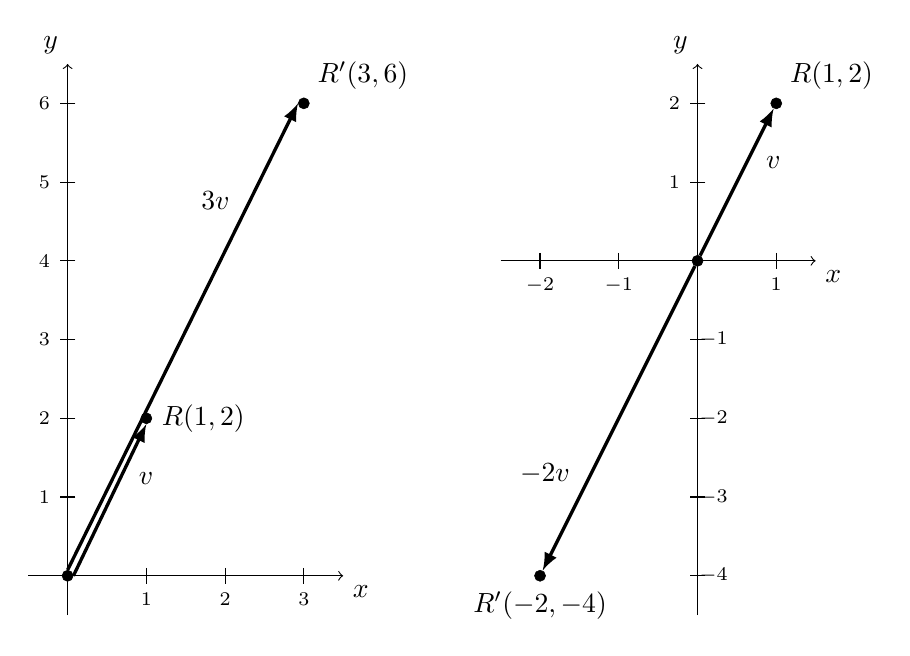
\begin{tikzpicture}[
	point/.style={circle,draw,very thin,fill,inner sep=0pt,minimum size=4pt},
	vector/.style={-latex},
]

	% 3x
	\begin{scope}
		\draw[->] (-0.5,0) to (3.5,0) node[below right] {$x$};
	  \draw[->] (0,-0.5) to (0,6.5) node[above left] {$y$};
		\foreach \x in {1,2,3} {
			\draw (\x,0.1) to (\x,-0.1) node[below] {$\scriptstyle \x$};
		}
		\foreach \y in {1,2,3,4,5,6} {
			\draw (0.1,\y) to (-0.1,\y) node[left] {$\scriptstyle \y$};
		}
		\node[point] at (0,0) (o) {};
		\node[point] at (1,2) (r) [label=right:{$R(1,2)$}] {};
		\node[point] at (3,6) (r2) [label=above right:{$R'(3,6)$}] {};
		\draw[vector,very thick] (o.north) to node[above left,near end] {$3\uvec{v}$} (r2.west);
		\draw[vector,very thick] (o.east) to node[below right,near end] {$\uvec{v}$} (r.south);
	\end{scope}

	% -2x
	\begin{scope}[xshift=8cm,yshift=4cm]
		\draw[->] (-2.5,0) to (1.5,0) node[below right] {$x$};
	  \draw[->] (0,-4.5) to (0,2.5) node[above left] {$y$};
		\foreach \x in {-2,-1,1} {
			\draw (\x,0.1) to (\x,-0.1) node[below] {$\scriptstyle \x$};
		}
		\foreach \y in {1,2} {
			\draw (0.1,\y) to (-0.1,\y) node[left] {$\scriptstyle \y$};
		}
		\foreach \y in {-4,-3,-2,-1} {
			\draw (0.1,\y) to (-0.1,\y) node[right] {$\scriptstyle \y$};
		}
		\node[point] at (0,0) (o) {};
		\node[point] at (1,2) (r) [label=above right:{$R(1,2)$}] {};
		\node[point] at (-2,-4) (r2) [label=below:{$R'(-2,-4)$}] {};
		\draw[vector,very thick] (o) to node[below right,near end] {$\uvec{v}$} (r);
		\draw[vector,very thick] (o) to node[above left,near end] {$-2\uvec{v}$} (r2);
	\end{scope}

\end{tikzpicture}
